\section{JPEG}
\begin{enumerate}
    \item Y Cr Cb Conversion
    \item 8x8 Pixel Blocks
    \item Discrete Cosine Transformation (DCT)
    \item Quantization
    \item Zig-Zag Scanning
    \item DC and AC Seperation
    \item Run-Length Encoding
    \item Huffman Encoding
    \item JFIF File Creation
\end{enumerate}
\subsection{y $C_r$ $C_b$ Conversion}
Das Bild wird  in Lumineszenz (Y) und Chrominanz ($C_r$, $C_b$) aufgeteilt.
$C_b$ ist der Blauanteil und $C_r$ der Rotanteil.
\subsubsection{Subsampling}
\begin{align*}
    R = \frac{\text{Resultierende Pixel}}{\text{Ursprüngliche Pixel}}
\end{align*}
\begin{itemize}
    \item Subsampling meint, dass in beiden Chrominanz-Ebenen in der
        Horizontalen oder Vertikalen mehrere Pixel zusammengefasst werden.
    \item Der Schema-Indikator gibt die Art des Subsamplings an und hat die
        Form J:a:b (z.B. 4:2:0)
    \item Diese Notation basiert auf einem Referenzbildblock, der J Pixel breit und
        2 Pixel hoch ist. Üblich ist J = 4.
\end{itemize}
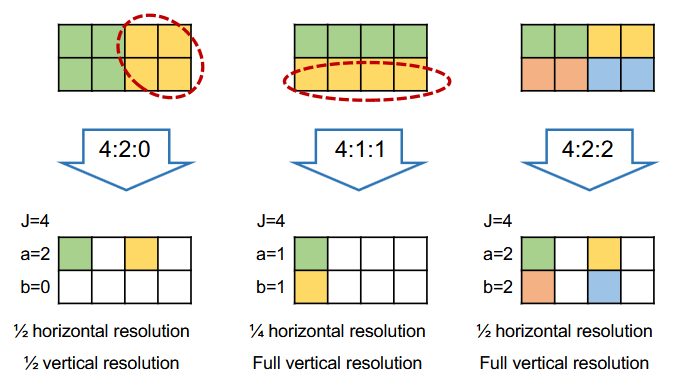
\includegraphics[scale=0.56]{subsampling1}\\
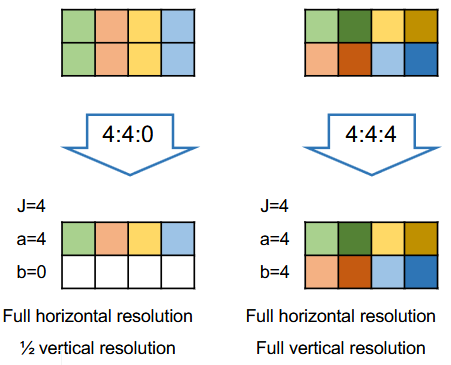
\includegraphics[scale=0.55]{subsampling2}

\subsection{8x8 Pixel Blocks}
Das Bild wird in 8x8 Pixel Blöcke aufgeteilt. Diese Blöcke werden dann einzeln bearbeitet.
\subsection{Discrete Cosine Transformation (DCT)}
Jeder wert der 8x8 Matrix wird durch die DCT in einen Frequenzraum transformiert.
\begin{equation*}
    F(u,v) = \frac{1}{4} \cdot C(u) \cdot C(v) \cdot \sum_{x=0}^{7} \sum_{y=0}^{7} f(x,y) \cdot \cos(\frac{(2x+1)u\pi}{16}) \cdot \cos(\frac{(2y+1)v\pi}{16})
\end{equation*}
Vor DCT:
\begin{center}
    \begin{tabular}{ c c c c c c c c c }
        139 & 144 & 149 & 153 & 155 & 155 & 155 & 155 \\
        144 & 151 & 153 & 156 & 159 & 156 & 156 & 156 \\
        150 & 155 & 160 & 163 & 158 & 156 & 156 & 156 \\
        159 & 161 & 162 & 160 & 160 & 159 & 159 & 159 \\
        159 & 160 & 161 & 162 & 162 & 155 & 155 & 155 \\
        161 & 161 & 161 & 161 & 160 & 157 & 157 & 157 \\
        162 & 162 & 161 & 163 & 162 & 157 & 157 & 157 \\
        162 & 162 & 161 & 161 & 163 & 158 & 158 & 158 \\
    \end{tabular}
\end{center}
Nach DCT ($Q_{vu}$):
\begin{center}
    \begin{tabular}{ c c c c c c c c }
        1260 & -1.0 & -12.1 & -5.2 & 2.1 & -1.7 & -2.7 & 1.3 \\
        -22.6 & -17.5 & -6.2 & -3.2 & -2.9 & -0.1 & 0.4 & -1.2 \\
        -10.9 & -9.3 & -1.6 & 1.5 & 0.2 & -0.9 & -0.6 & -0.1 \\
        -7.1 & -1.9 & 0.2 & 1.5 & 0.9 & -0.1 & -0.0 & 0.3 \\
        -0.6 & -0.8 & 1.5 & 1.6 & -0.1 & -0.7 & 0.6 & 1.3 \\
        1.8 & -0.2 & 1.6 & -0.3 & -0.8 & 1.5 & 1.0 & -1.0 \\
        -1.3 & -0.4 & -0.3 & -1.5 & -0.5 & 1.7 & 1.1 & -0.8 \\
        -2.6 & 1.6 & -3.8 & -1.8 & 1.9 & 1.2 & -0.6 & -0.4 \\
    \end{tabular}
\end{center}
\subsection{Quantization}
Die Frequenzanteile von der DCT werden nun durch eine Quantizationstabelle ($Q_{vu}$) geteilt. Die Quantizationstabelle
wird je nach JPEG Verfahren anders gewählt. Quantizationstabelle für Luminanz:
\begin{center}
    \begin{tabular}{ c c c c c c c c }
        16 & 11 & 10 & 16 & 24 & 40 & 51 & 61 \\
        12 & 12 & 14 & 19 & 26 & 58 & 60 & 55 \\
        14 & 13 & 16 & 24 & 40 & 57 & 69 & 56 \\
        14 & 17 & 22 & 29 & 51 & 87 & 80 & 62 \\
        18 & 22 & 37 & 56 & 68 & 109 & 103 & 77 \\
        24 & 35 & 55 & 64 & 81 & 104 & 113 & 92 \\
        49 & 64 & 78 & 87 & 103 & 121 & 120 & 101 \\
        72 & 92 & 95 & 98 & 
    \end{tabular}
\end{center}
Nun nimmt man die 8x8 Tabelle von nach der DCT und teilt sie durch die Quantizationstabelle bzw.
Folgende Funktion:
\begin{align*}
    F_{vu} = round(F_{vu}/Q_{vu})
\end{align*}

\begin{center}
    \begin{tabular}{ c c c c c c c c }
        79 & 0 & -1 & 0 & 0 & 0 & 0 & 0 \\
        -2 & -1 & 0 & 0 & 0 & 0 & 0 & 0 \\
        -1 & -1 & 0 & 0 & 0 & 0 & 0 & 0 \\
        -1 & 0 & 0 & 0 & 0 & 0 & 0 & 0 \\
        0 & 0 & 0 & 0 & 0 & 0 & 0 & 0 \\
        0 & 0 & 0 & 0 & 0 & 0 & 0 & 0 \\
        0 & 0 & 0 & 0 & 0 & 0 & 0 & 0 \\
        0 & 0 & 0 & 0 & 0 & 0 & 0 & 0
    \end{tabular}
\end{center}


